\documentclass[a4paper, 12pt,twoside]{article}
\usepackage[utf8]{inputenc}
\usepackage[frenchb,noconfigs]{babel}
\usepackage[T1]{fontenc}
\usepackage[scaled]{beramono}
\renewcommand*\familydefault{ttdefault}
\usepackage{listings}
\lstset{
  language=[GNU]C++,
  showstringspaces=false,
  formfeed=\newpage,
  tabsize=4,
  commentstyle=\itshape,
  basicstyle=\ttfamily,
  morekeywords={models, lambda, forms}
}

\newcommand{\code}[2]{
  \hrulefill
  \subsection*{#1}
  \lstinputlisting{#2}
  \vspace{2em}
}

\newcommand{\func}[1]{
\textbf{\texttt{#1}()}
}

\newcommand{\param}[1]{
\texttt{#1}
}

\usepackage{lmodern,textcomp,ifthen,graphicx,enumitem}
\usepackage[notes,
            titlepage,
            a4paper,
            pagenumber,
            sectionmark,
            twoside,
            fancysections]{polytechnique}
\usepackage[colorlinks=true,
            linkcolor=black,%bleu303,
            filecolor=red,
            urlcolor=bleu303,
            bookmarks=true,
            bookmarksopen=true]{hyperref}

\title{Détecteur de Viola Jones}
\subtitle{Projet \\ INF 442}
\author{
	Responsable du projet~: Jean Baptiste Bordes \\
        Felipe \textsc{Garcia} \\
        Francisco Eckhardt \\
        }
\date\today

\begin{document}
    \maketitle
    \renewcommand{\baselinestretch}{1.1}
    \setlength{\parskip}{0.5em}
    \tableofcontents
    \clearpage

%%%%%%%%%%%%%%%%%%%%%
%% DEBUT DU DOCUMENT %%%%%%
%%%%%%%%%%%%%%%%%%%%%
\section{Présentation du sujet}

	L’objectif de notre projet est d’implémenter un détecteur de visages basé sur les caractéristiques introduites par Viola et Jones. Pour cela, on utilise des vecteurs de caractéristiques qui correspondent à un grand nombre de régions et tailles différentes possibles qu’on calculera pour plusieurs images. On les utilise à la fin dans la prise de décision (détection). 
	
	Dans le cadre de l’analyse des images nous avons utilisé la bibliothèque Open Source \param{CImg} pour accéder aux pixels et transformer les fichiers \param{.jpg} en matrices de \param{long} en C++. Ces matrices sont converties en Images Intégrales pour un traitement postérieur.
	
	La deuxième partie de notre projet ce concentre sur la création des classifieurs qui discernent entre images de visages et de non visages. Nous avons utilisé l’algorithme du perceptron pour leur apprendre cette tâche. Ces résultats préliminaires sont ensuite pris par AdaBoost pour augmenter le pourcentage de détection de faces.
	
	Dans la phase finale ce centre sur la discussion de la précision de notre classifieur final en fonction du paramètre extérieur $\theta$ par une analyse de faux positifs et faux négatifs. Puis nous faisons une extension de notre algorithme pour repérer des visages dans des images quelconques.

\clearpage

%%%%%%%%%%%%%%%%%%%%%%%
%% EXPLICATION ALGORITHME %%%%%%
%%%%%%%%%%%%%%%%%%%%%%%
\section{Explication de l'algorithme}


\subsection{Calcul de l'Image Intégrale}
	
	On ouvre l’image avec l’aide de la bibliothèque \param{CImg} comme une matrice de \param{long}, on la parcourt une seule fois (fonction \func{SAT}), avec deux boucles \param{for}, l’une pour la hauteur et l’autre pour la largeur, en calculant l’image intégrale. On a utilisé la fonction \func{printData} pour en tester le bon fonctionnement dans le fichier \param{test\_q\_1\_1.cpp}.


\subsection{Définition des caractéristiques en parallèle}

	On a créé la classe auxiliaire feature pour représenter une caractéristique, avec les champs représentant position, largeur, hauteur et type de caractéristique (conforme à la Figure \ref{caracteristiques}).
	
	Pour créer des différentes caractéristiques, on a imposé aux côtés des rectangles une taille minimale de 8 pixels et on a pris un incrément minimal de position et de taille de  4 pixels. La fonction \func{distFeat} lance 4 threads responsables de créer les caractéristiques de chaque type (‘a’, ‘b’, ‘c’ et ‘d’), puis les retourne dans un même vecteur. On a ainsi obtenu 128227 caractéristiques au total.


%%%%%%%%%%%%%
%% IMAGE %%%%%%
%%%%%%%%%%%%%
\begin{figure}[htbp]
\centering
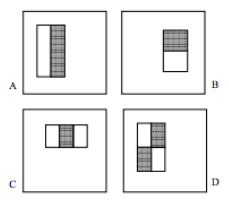
\includegraphics[scale=0.8]{charact}
\caption{Types des caractéristiques utilisées}
\label{caracteristiques}
\end{figure}
%%%%%%%%%%%%%
%%%END IMAGE%%%%
%%%%%%%%%%%%%

\subsection{Entraînement des classifieurs faibles en parallèle}

	À chaque caractéristique on associe un classifieur faible ($h_i$, représentés par la classe auxiliaire classifier, avec deux paramètres $w_1$ et $w_2$ et la fonction \param{calc(x)} qui renvoie $h(x)$, conforme défini dans le sujet). Chaque classifieur faible est entraîné en utilisant la méthode du Perceptron.
	
	Les fonctions auxiliaires \func{readImgs} et \func{distII} sont responsables d’ouvrir et de calculer l’image intégrale des images d’un répertoire de manière parallélisée, ce qu’on a utilisé pour les trois répertoires “Train”, “Validation” et “Test”. De même pour l’entraînement : on distribue entre les \param{threads} différents classifieurs pour qu’ils les travaillent parallèlement.


\subsection{Boosting et choix de classifieurs}

	On utilise l’algorithme Adaboost pour créer un classifieur final en utilisant une combinaison linéaire de classifieurs faibles précédemment définies. L’idée consiste en donner plus de poids pour les classifieurs les plus performants et ainsi obtenir un classifieur final qui les prend en compte de façon pondérée. Les étapes de choix du classifieur faible et de mise à jour des poids ($\lambda_i $ pour $ i \in \{1, \ldots, n\}$) sont faites en parallèle.

\clearpage

%%%%%%%%%%%%%%%%%%%%%%%
%% TEST DES RÉSULTATS %%%%%%
%%%%%%%%%%%%%%%%%%%%%%%

\section{Test et Analyse des résultats}

\subsection{Variation en fonction du paramètre $\theta \in [-1,1]$}

	On a créé un programme pour tester la performance de notre classifieur F en fonction de $\theta$ en calculant le taux de faux négatifs et faux positifs dans un intervalle [$\theta_{min}$, $\theta_{max}$] choisi par l'utilisateur. Les autres paramètres peuvent aussi être modifiés dans le code.

\subsection{Extension de l’algorithme}

	Notre algorithme est prêt à calculer l'Image Intégrale d'images de n'importe quelle taille. Pour l'adapter il faut donc suivre l'approche proposé par Viola et Jones ([4]) de redimensionner les caractéristiques au lieu de redimensionner les images et les faire parcourir toute l'image.
\clearpage
 
%%%%%%%%%%%%%%
%%    BIBLIOGRAFIA %%
%%%%%%%%%%%%%%

\section{Références bibliographiques}
        {
        \renewcommand{\section}[2]{} % pour virer le titre "Références"
        \nocite{*} %% INCLUDE ALL BIB
        \bibliographystyle{plain}
        \bibliography{Rapport_VJ.bib}
        }
        
%%%%%%%%%%%%%%%%%%%%%
%% FIN DU DOCUMENT %%%%%%
%%%%%%%%%%%%%%%%%%%%%
    
\end{document}
